%%%%%%%%%%%%%%%%%%%%%%%%%%%%%%%%%%%%%%%%%%%%%%
%%%%%%%%%%%%%%%%%%%%%%%%%%%%%%%%%%%%%%%%%%%%%%
%%                                          %%
%% Important note on usage                  %%
%% -----------------------                  %%
%% This file must be compiled with PDFLaTeX %%
%% Using standard LaTeX will not work!      %%
%%                                          %%
%%%%%%%%%%%%%%%%%%%%%%%%%%%%%%%%%%%%%%%%%%%%%%
%%%%%%%%%%%%%%%%%%%%%%%%%%%%%%%%%%%%%%%%%%%%%%

%% The '3p' and 'times' class options of elsarticle are used for Elsevier CRC
% \documentclass[5p]{elsarticle}
% Good for final formatting  - two column
% 
% \documentclass[3p,times]{elsarticle}
\documentclass[3p]{elsarticle}
% Good for proofing - single column
% 

\usepackage[american]{babel}
\usepackage{amsmath}
\usepackage[version=3]{mhchem} 
% \usepackage{fixltx2e}
% \usepackage{refcount}
% \usepackage{siunitx}
% \usepackage{lastpage}
% \usepackage{textcomp}
\usepackage{mathtools}

\usepackage{xfrac}
\usepackage{lmodern}
\usepackage[hidelinks]{hyperref}
% \usepackage{cool}
% \usepackage{cancel}
\usepackage{microtype}
\usepackage{listings}
\usepackage{mcode}
\usepackage [autostyle, english = american]{csquotes}
\usepackage{longtable}
\usepackage{subcaption}
\usepackage{booktabs,siunitx}
\usepackage{gensymb}
\usepackage[normalem]{ulem}

% \usepackage{mathtools, cuted}


% \usepackage[usenames,dvipsnames,svgnames,table]{xcolor}
\usepackage{color}

\usepackage[colorinlistoftodos]{todonotes}

\usepackage[section]{placeins}
\usepackage{multirow}

\usepackage{lineno}



\lstset{basicstyle=\small\ttfamily,columns=fullflexible}

% \usepackage{verbatim}



% \usepackage{gensymb}
% \usepackage{enumerate}
% \usepackage{float}
% \usepackage{bm}
% \usepackage{csquotes}
% \usepackage{mathtools}
% \usepackage{natbib}
% \usepackage{biblatex}

%% The `ecrc' package must be called to make the CRC functionality available
\usepackage{ecrc}

%% The ecrc package defines commands needed for running heads and logos.
%% For running heads, you can set the journal name, the volume, the starting page and the authors

%% set the volume if you know. Otherwise `00'
\volume{00}

%% set the starting page if not 1
\firstpage{1}

%% Give the name of the journal
\journalname{Nuclear Instruments and Methods in Physics Research B}

%% Give the author list to appear in the running head
%% Example \runauth{C.V. Radhakrishnan et al.}
\runauth{A.S. Voyles et al.}

%% The choice of journal logo is determined by the \jid and \jnltitlelogo commands.
%% A user-supplied logo with the name <\jid>logo.pdf will be inserted if present.
%% e.g. if \jid{yspmi} the system will look for a file yspmilogo.pdf
%% Otherwise the content of \jnltitlelogo will be set between horizontal lines as a default logo

%% Give the abbreviation of the Journal.
\jid{nimb}
% \jid{yspmi}

%% Give a short journal name for the dummy logo (if needed)
\jnltitlelogo{Nucl Instrum Meth B}

%% Hereafter the template follows `elsarticle'.
%% For more details see the existing template files elsarticle-template-harv.tex and elsarticle-template-num.tex.

%% Elsevier CRC generally uses a numbered reference style
%% For this, the conventions of elsarticle-template-num.tex should be followed (included below)
%% If using BibTeX, use the style file elsarticle-num.bst

%% End of ecrc-specific commands
%%%%%%%%%%%%%%%%%%%%%%%%%%%%%%%%%%%%%%%%%%%%%%%%%%%%%%%%%%%%%%%%%%%%%%%%%%

%% The amssymb package provides various useful mathematical symbols
\usepackage{amssymb}
%% The amsthm package provides extended theorem environments
\usepackage{amsthm}

%% The lineno packages adds line numbers. Start line numbering with
%% \begin{linenumbers}, end it with \end{linenumbers}. Or switch it on
%% for the whole article with \linenumbers after \end{frontmatter}.
%% \usepackage{lineno}

%% natbib.sty is loaded by default. However, natbib options can be
%% provided with \biboptions{...} command. Following options are
%% valid:

%%   round  -  round parentheses are used (default)
%%   square -  square brackets are used   [option]
%%   curly  -  curly braces are used      {option}
%%   angle  -  angle brackets are used    <option>
%%   semicolon  -  multiple citations separated by semi-colon
%%   colon  - same as semicolon, an earlier confusion
%%   comma  -  separated by comma
%%   numbers-  selects numerical citations
%%   super  -  numerical citations as superscripts
%%   sort   -  sorts multiple citations according to order in ref. list
%%   sort&compress   -  like sort, but also compresses numerical citations
%%   compress - compresses without sorting
%%
%% \biboptions{comma,round}

% \biboptions{}

% if you have landscape tables
\usepackage[figuresright]{rotating}

% put your own definitions here:
%   \newcommand{\cZ}{\cal{Z}}
%   \newtheorem{def}{Definition}[section]
%   ...

% add words to TeX's hyphenation exception list
%\hyphenation{author another created financial paper re-commend-ed Post-Script}

% declarations for front matter

\usepackage{fancyvrb}
\usepackage{color}
 
\definecolor{mygreen}{rgb}{0,0.6,0}
\definecolor{mygray}{rgb}{0.5,0.5,0.5}
\definecolor{mymauve}{rgb}{0.58,0,0.82}

\lstset{ %
  backgroundcolor=\color{white},   % choose the background color
  basicstyle=\footnotesize,        % size of fonts used for the code
  breaklines=true,                 % automatic line breaking only at whitespace
  captionpos=b,                    % sets the caption-position to bottom
  commentstyle=\color{mygreen},    % comment style
  escapeinside={\%*}{*)},          % if you want to add LaTeX within your code
  keywordstyle=\color{blue},       % keyword style
  stringstyle=\color{mymauve},     % string literal style
}

% Sin and Cos with auto-parentheses 
\newcommand{\sinp}[1]{\sin{\left( #1\right)}}
\newcommand{\cosp}[1]{\cos{\left( #1\right)}}
\newcommand{\expp}[1]{\exp{\left( #1\right)}}
\newcommand{\sinhp}[1]{\sinh{\left( #1\right)}}
\newcommand{\lnp}[1]{\ln{\left( #1\right)}}
\newcommand{\pp}[1]{\left( #1\right)}
\newcommand{\sci}[2]{ #1 \cdot 10^{#2}\ }
\newcommand{\angstrom}{\mbox{\normalfont\AA}}
\newcommand{\norm}[1]{\lVert #1 \rVert}

\newcommand{\textred}[1]{\textcolor{red}{ #1}}
\newcommand{\redactedit}[1]{\textcolor{blue}{ \sout{#1}}}


\newcommand{\colornote}[1]{\textcolor{red}{ COMMENT\large\footnote{\textcolor{red}{#1}}}}

\newcommand{\comment}[1]{\todo[color=blue!20!white,inline]{ASV: #1}} 

% Tweak sim for better inline text tilde
\newcommand{\mytilde}{\raisebox{0.5ex}{\texttildelow}}
% \newcommand{\mytilde}{\raise.17ex\hbox{$\scriptstyle‌​\sim$}}

\sisetup{separate-uncertainty=true,table-space-text-post = *}

\newcommand{\minitab}[2][l]{\begin{tabular}{#1}#2\end{tabular}}

\newcommand{\subfigimg}[3][,]{%
  \setbox1=\hbox{\includegraphics[#1]{#3}}% Store image in box
  \leavevmode\rlap{\usebox1}% Print image
  \rlap{\hspace*{50pt}\raisebox{\dimexpr\ht1-2\baselineskip}{#2}}% Print label
  \phantom{\usebox1}% Insert appropriate spcing
}


\makeatletter
% Make common definition of mean
\newcommand*\mean[1]{\overline{#1\raisebox{3mm}{}}}

\makeatother


\begin{document}

\begin{frontmatter}

%% Title, authors and addresses

%% use the tnoteref command within \title for footnotes;
%% use the tnotetext command for the associated footnote;
%% use the fnref command within \author or \address for footnotes;
%% use the fntext command for the associated footnote;
%% use the corref command within \author for corresponding author footnotes;
%% use the cortext command for the associated footnote;
%% use the ead command for the email address,
%% and the form \ead[url] for the home page:
%%
\title{Measurement of nuclear excitation functions for proton induced reactions (E$_{\text{p}}$ = 40 -- 90 MeV) on Nb and Cu}

%% \tnotetext[label1]{}
%% \author{Name\corref{cor1}\fnref{label2}}
%% \ead{email address}
%% \ead[url]{home page}
%% \fntext[label2]{}
%% \cortext[cor1]{}
%% \address{Address\fnref{label3}}
%% \fntext[label3]{}

% \dochead{Short}
%% Use \dochead if there is an article header, e.g. \dochead{Short communication}


% \author[rvt]{C.V. ̃Radhakrishnan\corref{cor1}\fnref{fn1}}
\author[ucb]{Andrew S. Voyles \corref{cor1}}
\ead{andrew.voyles@berkeley.edu}

% \author[lbl]{M.S. Basunia}
% 
% \author[ucb]{J.C. Batchelder}
% 
% \author[llnl]{J.D. Bauer}
% 
% \author[geo]{T.A. Becker}


\author[ucb,lbl]{Lee A. Bernstein}


\author[lanl]{Eva R. Birnbaum}

\author[uwm]{Jonathan W. Engle}

\author[iowa]{Stephen A. Graves}

\author[ucb]{Amanda M. Lewis}


\author[lanl]{Francois M. Nortier}

% \author[ucb]{M.A. Unzueta}
% 
% \author[ucb]{K.A. van Bibber}



%% use optional labels to link authors explicitly to addresses:
%% \author[label1,label2]{<author name>}
%% \address[label1]{<address>}
%% \address[label2]{<address>}

\cortext[cor1]{Corresponding author}
% \cortext[cor2]{Principal corresponding author}
% \fntext[fn1]{This is the specimen author footnote.}
% \fntext[fn2]{Another author footnote, but a little more longer.}

% \address[ucb]{Department of Nuclear Engineering, University of California, Berkeley, Etcheverry Hall, 2521 Hearst Ave, Berkeley, CA 94709}
% \address[lbl]{Lawrence Berkeley National Laboratory,  1 Cyclotron Rd, Berkeley, CA 94720}
% \address[llnl]{Lawrence Livermore National Laboratory, 7000 East Ave, Livermore, CA 94550}

\address[ucb]{Department of Nuclear Engineering, University of California, Berkeley, 4155 Etcheverry Hall, MC 1730, Berkeley, CA 94720, USA}
\address[lbl]{Lawrence Berkeley National Laboratory, 1 Cyclotron Rd., Berkeley, CA 94720, USA}
% \address[llnl]{Lawrence Livermore National Laboratory, Livermore CA, 94551 USA}
% \address[geo]{Berkeley Geochronology Center, Berkeley CA,  94709  USA}
\address[uwm]{Department of Medical Physics, University of Wisconsin -- Madison, 1111 Highland Ave., Madison, WI 53705, USA}
\address[lanl]{Los Alamos National Laboratory, P.O. Box 1663, Los Alamos, NM 87544, USA}
\address[iowa]{Department of Radiation Oncology, University of Iowa, 200 Hawkins Drive, Iowa City, IA 52242, USA}




\begin{abstract}







XXXXX




% Cross sections for the \ce{^{47}Ti}(n,p)\ce{^{47}Sc} and \ce{^{64}Zn}(n,p)\ce{^{64}Cu} reactions have been measured for quasi-monoenergetic DD neutrons produced by the UC Berkeley High Flux Neutron Generator.
% The study was motivated by interest in the production of \ce{^{47}Sc} and \ce{^{64}Cu} as emerging medical isotopes.
% The cross sections were measured in ratio to the \ce{^{113}In}(n,n')\ce{^{113m}In} and \ce{^{115}In}(n,n')\ce{^{115m}In} inelastic scattering reactions on co-irradiated indium samples.
% Post-irradiation counting using an HPGe and LEPS detectors allowed for cross section determination to within 5\% uncertainty.
% The cross sections were determined with lower uncertainty than existing measurements and are found to be  in good agreement with both empirical and theoretical values.
% This work highlights the utility of using DD plasma-based neutron sources for a host of nuclear data measurements and potentially for the production of radionuclides for medical applications.

% \comment{Karl:  \enquote{Comment to engender some discussion.  I have a small concern here, reminiscent of what happened to our electron backstreaming paper in PRAB.  To be publishable, even in NIMB, there has to be a crisp research question resolved, or some innovation.  I think an angle that is missing here is that this is a new design of neutron generator, whose design maximizes the flux density (n/sec/cm2), although the total flux, while respectable, is not spectacular in itself.  This is Lee's recent mantra, and I now understand its significance.  Problematically, as Andrew has pointed out, we don't have the actual instrument paper published yet, so the thrust of the paper can't be too focused on the flux density issue, but a workable angle would be \enquote{given we have this new capability, this is an example of its power}.  Let me suggest Lee provide a sentence for the abstract, and a few sentences of text in the appropriate spot.}}

% \comment{The abstract is now nicely short and sweet, but should it be expanded at all?}



\end{abstract}

\begin{keyword}
%% keywords here, in the form: keyword \sep keyword
Nb+p \sep Cu+p \sep Niobium \sep Copper\sep Aluminum \sep Nuclear cross sections \sep Proton activation \sep Proton transport \sep Stacked target activation \sep Monitor foils \sep Medical isotope production \sep MCNP \sep  LANL

%% MSC codes here, in the form: \MSC code \sep code
%% or \MSC[2008] code \sep code (2000 is the default)

\end{keyword}

\end{frontmatter}

%%
%%  To-do list for comments
%%
\listoftodos


%%
%% Start line numbering here if you want
%%
\linenumbers



%% main text 
\section{Introduction} \label{sec:intro}

% \comment{cite theranostic papers, etc}

Every year, approximately 17 million nuclear medicine procedures (both diagnostic and therapeutic) are performed in the U.S. alone - a multi-billion dollar industry which has made incredible strides in improving our ability to detect and treat a variety of life-threatening diseases \cite{Delbeke2011,NSACIsotopesSubcommittee2015}.
The vast majority of the radioisotopes currently used for these procedures are produced in the field's array of low- (E \textless\ 30 MeV / A) and intermediate-energy (30 \textless\ E \textless\ 200 MeV / A) accelerator capabilities, which routinely produce many of the staple medical radionuclides, such as \ce{^{18}F} \ce{^{68}Ge}, \ce{^{82}Rb}, and \ce{^{123}I}, as well as many of the non-medical radioisotopes of commercial value, such as  \ce{^{32}Si}, \ce{^{73}As}, \ce{^{95m}Tc}, and  \ce{^{109}Cd} \cite{international2009iaea,schlyer2008cyclotron}. 
\comment{Should \enquote{intermediate-energy} be less than 200 MeV, or 100 MeV?  I find conflicting descriptions in the literature.}
 The future of nuclear medicine would appear to be the paradigm of personalized medicine - targeted radionuclide therapy to spare healthy tissue \cite{Mulford2005,Qaim201731}, and theranostic medicine, which pairs an imaging isotope with a therapeutic isotope of the same element, to provide simultaneous, real-time dose delivery and verification, leading to drastic reductions in prescribed patient dose \cite{Muller2014,Bentzen2005,Srivastava2012}. 
Candidate isotopes to fill these needs have been identified based on their decay properties \cite{NSACIsotopesSubcommittee2015,Qaim201731,bernstein2015nuclear}, and a series of campaigns are underway to perform targeted, high-priority measurements of thin-target cross sections and thick-target integral yields, to facilitate production in sufficient quantities for cell studies.


However, one significant obstacle exists for both high-fidelity measurements of emerging medical radionuclides, as well as conventional isotope production: well-characterized  dosimetry standards.  
This is particularly true for intermediate-energy charged particle beams, where there is currently a paucity of such well-characterized data. 
Indeed, the development of new dosimetry standards and the improved evaluation of existing standards is one of the areas of greatest cross-cutting need for nuclear data \cite{bernstein2015nuclear}. 
Charged particle dosimetry data currently exists for low-to-intermediate energy charged particle beams (E \textless\ 50 MeV / A), but experimental data used for this evaluation is sparse above approximately 30 MeV / A and  uncertainties in experimental cross sections are large (6-15\%) \cite{gul2001charged}. 
While work is needed to improve upon existing dosimetry data, the development of new dosimetry reactions can expand the available range of options for the monitoring of charged particle beams.


Activation is one of the most fundamental techniques utilized in experimental nuclear physics, as it is a simple and straightforward method to probe the structure and behavior of nuclear matter,  dating back to the infancy of the field. 
While the specifics have branched into ever-more-detailed probes into the world of the nucleus, activation, at heart, deals with the analysis and quantification of decaying radioactive nuclei created through irradiation via ionizing radiation \cite{ehmann1993radiochemistry,krüger1971principles}.
Monitor reactions have  historically been part of such activation experiments, and in the context of charged particle induced reactions, serve two valuable purposes, depending upon the energy regime in question.  
Between the reaction's energetic threshold  and the tail of its compound peak, the magnitude and shape of a monitor reaction's excitation function is rapidly changing with increasing incident particle energy.
In this energy regime, a monitor reaction can be used to assign an energy bin to a thin irradiated target, especially when comparing between monitor reactions leading to two distinct residual nuclei from the same target, such as the $^\text{nat}$Cu(p,x)\ce{^{62}Zn} and $^\text{nat}$Cu(p,x)\ce{^{63}Zn} reactions \cite{gul2001charged}.
This is extremely useful, as it allows one to screen for and eliminate systematic errors based on energy assignment, though this sensitivity to energy precludes their reliability as a beam current monitor.  

Moving to the higher energy  of the reaction's pre-equilibrium tail, the excitation function becomes  smooth and generally flat as a function of energy.
In this regime, the monitor reaction offers little-to-no energy sensitivity. 
In return for giving up the ability to assign energy positions, monitor reactions in the pre-equilibrium regime become extremely useful for monitoring the integral beam current incident upon the target. 
While cross section measurements often use external beam current monitors (such as an inductive pickup upstream of a target, or electrically-isolated target in a Faraday cup), these measure the integrated current incident upon an entire target assembly.
For the case of stacked-target activation experiments, commonly employed to measure cross sections at multiple energy positions in a single activation, external beam current monitors can only measure the integral current incident upon the \enquote{front} (upstream) of the target stack.
In these experiments, a series of monitor foils at each energy position allow one to measure the integral current at each position in the stack, reducing systematic errors in observed cross section magnitude.
Both of these purposes make well-characterized dosimetry an invaluable asset to any activation experiment. 



In practice, nearly any radioisotope can serve as a reaction monitor. 
However, several characteristics are hallmarks of a reaction monitor worthy to be classified as a dosimetry standard.
The primary factor involved in selecting a new monitor is ensuring that the desired radionuclide has  at least one (preferably multiple, to ensure accurate radionuclide identification) distinct decay radiation able to used to uniquely identify it during post-activation assay.  
Generally, this means selecting a radionuclide with a number of distinct gamma rays, as gamma spectroscopy is commonly used to identify and quantify reaction products.
The decay radiation should preferably have high intensities, so that they show up as strong peaks during spectroscopy, and minimize the amount of time needed to count the activated target in order to achieve acceptable counting statistics. 

Care should be taken to avoid cases where a radionuclide which is one decay off of stability populates excited states in the excited daughter nucleus also populated in the decay to the daughter state from the opposite side of the valley of stability.
This produces decay gamma rays with nearly exactly the same energy, making it difficult to disentangle production from both sides of stability.
For example, $^\text{nat}$Ti(p,x)\ce{^{48}V} is commonly used as dosimetry for 5 \textless\ E \textless\ 30 MeV protons.
The characteristic decay lines in \ce{^{48}V}  ($t_{1/2}$ = 15.97 d, $\epsilon=100\%$ to \ce{^{48}Ti}) are the 983.525 keV ($I_\gamma=99.98\%$) and 1312.106 keV ($I_\gamma=98.2\%$) gammas, which are also seen in the decay of \ce{^{48}Sc}  ($t_{1/2}$ = 43.67 h, $\beta^-=100\%$ to \ce{^{48}Ti}), yielding  a 983.526 keV ($I_\gamma=100.1\%$) and 1312.120 keV ($I_\gamma=100.1\%$) line \cite{Burrows2006}.
Fortunately, these cases can occasionally be mitigated by either using a difference in half-life between the two feeding pathways to allow one to decay out, or by using a distinct gamma ray from one of the two isobar nuclei to subtract out the activity associated with it (such as the $E_\gamma=1037.522$ keV,$I_\gamma=97.6\%$ line in the decay of \ce{^{48}Ti}) \cite{Burrows2006}.
However, this approach propagates larger uncertainties into the final activity of the desired monitor nucleus, so in principle it is far preferred to choose a monitor reaction which does not have overlapping gamma rays from another isobar nucleus.

Another important decay factor to consider is that of the half-life of the desired monitor nucleus.
It is preferred that the nucleus have a lifetime which is sufficiently long-lived to ensure that it may be quantified  conveniently and leisurely after end-of-beam without the majority if it decaying away.
In addition, it is preferred that the lifetime be comparable to that of the reaction products being studied. 
For proper quantification, it is also of vital importance that the proposed monitor nucleus have well-characterized decay data.
A precise and well-established half-life is needed to properly correct for decay losses during production, as well as in between end-of-beam and the start of decay spectroscopy, but these are generally well-characterized.
In practice, the weakest components of decay data are often the gamma ray intensities, which can routinely have uncertainties of 5\% or more.
Since this uncertainty is propagated in quadrature from the activity of both the monitor reaction and the reaction product being studied, choosing a monitor with a well-established gamma ray intensity can make a significant reduction in measured cross section uncertainties.
It is also of utmost importance to choose a reaction channel which cannot be populated via secondary particles incident upon the monitor target.
This is typically mostly a concern for secondary neutrons produced through (z,xn) reactions on upstream targets, degraders, and stack materials, to avoid monitor reactions which can be populated through (n,x) reactions on the target.
Any monitor reaction channel which can be populated by anything other than the primary beam should be avoided, as it is often a laborious task to separate out the fraction of secondary particles contributing to the total activation.  



Finally, from a targetry  perspective, it is preferable to use a target that is readily commercially available at an affordable price and is generally chemically inert - any significant chemical changes during target preparation (rapid oxidation, etc) will affect the target's areal density, systematically changing the measured integral current. 
Structurally, the target material should be malleable and supportive to be able to be formed into a thin target.
For charged particle reactions, a thin target is desired for dosimetry, as thicker targets will cause more energy degradation and broaden the energy spectrum downstream of the target.
% These are the primary characteristics involved in choosing an appropriate target for a monitor reaction




% The purpose of the present work is to explore the potential to use high-flux neutron generators to produce high-specific activity samples of radionuclides at the mCi level for local use in the application community. 
%  The research group at UC Berkeley has  developed a High Flux Neutron Generator (HFNG) that features an internal target where samples can be placed just several millimeters from the neutron producing surface in order to maximize the utilization of the neutron yield for the production of a desired radionuclide \cite{Waltz2017,Waltz2016a,doi:10.1063/1.3267832}.
%  The HFNG uses the D(D,n)\ce{^3He} reaction to produce neutrons with energies near 2.45 MeV together with a self-loading target design to maintain continuous operation without target replacement.
%  In addition to the generator itself, efforts are underway to design neutron reflection capabilities to allow scattered neutrons multiple opportunities to interact with an  internally mounted target.
% While these design efforts are underway, the HFNG can be used to better characterize production cross sections at the appropriate neutron energy.
% 
% 
% The present work features a pair of cross section measurements for the production of two emerging non-standard medical radionuclides: the positron emitter \ce{^{64}Zn}(n,p)\ce{^{64}Cu} and the single - photon emission computed tomography (SPECT) tracer \ce{^{47}Ti}(n,p)\ce{^{47}Sc}.
% \ce{^{64}Cu}  ($t_{1/2}$ = 12.7 h) undergoes $\beta^+$ decay (61.5\% branching ratio) to \ce{^{64}Ni} or $\beta^-$ decay (38.5\% branching ratio) to \ce{^{64}Zn} \cite{Singh2007}.
% The emitted short-range 190-keV $\beta^-$ particle makes this an  attractive  therapeutic radionuclide, which also has the possibility for simultaneous positron emission tomography (PET) imaging for real-time dose monitoring and verification.
% This makes \ce{^{64}Cu} particularly desirable  for emerging radiation therapy protocols \cite{Lewis2003,NSACIsotopesSubcommittee2015,Bandari2014,mp500671j}.
% In addition, copper radiochemistry is well developed, and many existing ligands and carriers may be used for selective delivery of the radionuclide to different sites in patients.
% The second radionuclide studied, \ce{^{47}Sc} ($t_{1/2}$ = 3.35 d), undergoes $\beta^-$ decay to \ce{^{47}Ti}, emitting a high-intensity (63.8\%) 159-keV gamma ray in the process \cite{Burrows2007}.
% This radionuclide is  attractive as an emerging diagnostic isotope, due to the similarity of the emitted gamma ray to that of the  well-established \ce{^{99m}Tc} \cite{Qaim2011,Qaim201731,Kolsky1998,mausner1995evaluation}.
% Due to the short half-life ($t_{1/2}$ = 6.0 h) of and dwindling supplies of \ce{^{99m}Tc}, \ce{^{47}Sc} stands poised as a potential solution to this shortage, due to its longer half-life and multiple production pathways without the need for highly enriched uranium \cite{Browne2011}.
% In addition, when paired with \ce{^{44}Sc}, \ce{^{47}Sc} forms a promising \enquote{theranostic} pair for use in simultaneous therapeutic and diagnostic applications \cite{Muller2014,Deilami-nezhad2016}.

% \comment{cite theranostic papers, etc}


One monitor reaction which satisfies these requirements is that of a new, intermediate-energy proton dosimetry standard based on \ce{^{93}Nb}(p,4n)\ce{^{90}Mo}. 
Niobium is naturally monoisotopic, readily  available commercially in high purity, is chemically inert, and can easily be rolled down to foils as thin as 1 $\micro$m.  
\ce{^{90}Mo} also has excellent decay properties - its fairly long-lived half-life ($\epsilon=100\%, t_{1/2}=5.56 \pm 0.09$ h) allows it to be counted at leisure without fear of the product \ce{^{90}Mo} decaying away excessively between end-of-beam and the start of counting, and it possesses seven strong, distinct gamma lines (notably its 122.370 keV ($I_\gamma = 64 \pm 3\%$) and 257.34 keV ($I_\gamma = 78 \pm 4\%$) lines) which can be used to uniquely and easily   quantify \ce{^{90}Mo} production \cite{Browne1997}. 
In addition,  \ce{^{90}Mo} is completely immune from (n,x) production on  \ce{^{93}Nb}, being produced only via the primary proton beam, and the \ce{^{90}Mo} decay lines can only be observed in its decay, as its daughter, \ce{^{90}Nb}, is also unstable and decays via $\epsilon$ to stable \ce{^{90}Zr}. 
 
The purpose of the present work is to  measure the production of the long-lived radionuclide \ce{^{90}Mo} ($t_{1/2}=5.56 \pm 0.09$ h \cite{Browne1997}) via the $^\text{nat}$Nb(p,x) reaction. 
In addition to the $^\text{nat}$Nb(p,x)\ce{^{90}Mo} measurement, this experiment has also yielded measurements of 32 other (p,x) production cross sections between 40 -- 90 MeV  for a number of additional reaction products, including several emerging radionuclides with medical applications.
These include the non-standard positron emission tomography (PET) emitters \ce{^{57}Ni}  ($t_{1/2}=35.60\pm0.06$ h \cite{Bhat1998}),  \ce{^{86}Y}  ($t_{1/2}=14.74\pm0.02$ h \cite{NEGRET20151}), \ce{^{89}Zr} ($t_{1/2}=78.41\pm0.12$ h \cite{Singh2013}),  \ce{^{90}Nb} ($t_{1/2}=14.60 \pm 0.05$ h \cite{Browne1997}), the $\beta^-$-therapy agent  \ce{^{64}Cu} ($t_{1/2}=12.701 \pm 0.002$ h \cite{Singh2007}),  and the Auger-therapy agent \ce{^{82\text{m}}Rb} ($t_{1/2}=6.472\pm0.006$ h \cite{Tuli2003}). 


  \comment{The following paragraph should only be included if we decide to touch on spin physics in this manuscript, or split it into a follow-on PhysRev C, etc.}

  
Measurements of isomer-to-ground state ratios have been used for over 20 years to probe the spin distribution of excited nuclear states in the A$\approx$ 190 region \cite{PhysRevC.73.034613,PhysRevC.45.1171}.
In addition to the interest in the production of \ce{^{90}Mo} as an intermediate-energy dosimetry standard, this experiment offers an opportunity to study the distribution of angular momentum in compound nuclear and direct pre-equilibrium reactions via observation of a number of isomer-to-ground state ratios.
These include the \ce{^{52\text{m}}Mn} ($t_{1/2}=21.1\pm0.2$ m; J$^\pi=2^+$) to \ce{^{52\text{g}}Mn}  ($t_{1/2}=5.591\pm0.003$ d; J$^\pi=6^+$), \ce{^{58\text{m}}Co} ($t_{1/2}=9.10\pm0.09$ h; J$^\pi=5^+$) to \ce{^{58\text{g}}Co}  ($t_{1/2}=70.86\pm0.06$ d; J$^\pi=2^+$),  \ce{^{85\text{m}}Y} ($t_{1/2}=4.86\pm0.13$ h; J$^\pi=\sfrac{9}{2}^+$) to \ce{^{85\text{g}}Y}  ($t_{1/2}=2.68\pm0.05$ h; J$^\pi=\sfrac{1}{2}^-$),  \ce{^{87\text{m}}Y} ($t_{1/2}=13.37\pm0.03$ h; J$^\pi=\sfrac{9}{2}^+$) to \ce{^{87\text{g}}Y}  ($t_{1/2}=79.8\pm0.3$ h; J$^\pi=\sfrac{1}{2}^-$),  and \ce{^{89\text{m}}Nb} ($t_{1/2}=66\pm2$ m; J$^\pi=\sfrac{1}{2}^-$) to \ce{^{89\text{g}}Nb}  ($t_{1/2}=2.03\pm0.07$ h; J$^\pi=\sfrac{9}{2}^+$)  ratios \cite{Dong2015,Nesaraja2010,Singh2014,Johnson2015,Singh2013}.  
 
 
This measurement has taken place using a set of multiple monitor reactions in conjunction with statistical calculations and proton transport simulations to reduce systematic uncertainties in beam energy assignments, leading to some of the first and most precise measurements  for many of the excitation functions reported here. 
By expanding the available set of dosimetry standards and well-characterized isotope production excitation functions, great advances are possible for improving the  available options for modern medical imaging and cancer therapy.

 
 
 


\section{Experimental methods and materials}\label{sec:experiment}



\subsection{Stacked-target design }\label{sec:target_design}

% \comment{Regex to replace all hard figure references with LaTeX cross-references  [F,f]igure[^s*}]     }

The well-known stacked-target design was utilized for this work, in order that the (p,x) cross sections for each reaction channel could be measured at multiple energy positions in a single irradiation \cite{Graves2016}. 
For targets, a series of nominal 25 \micro m \ce{^{nat}Nb} foils (99.8\%, lot \#T23A035), 25 \micro m \ce{^{nat}Al} foils (99.999\%, lot \#M06C032), and 50 \micro m \ce{^{nat}Cu} foils (99.9999\%, lot \#N26B062) were used (all from Alfa Aesar, Ward Hill, MA, 01835, USA).
Six foils of each metal were cut down to 2.5 x 2.5 cm squares and characterized - for each foil, length and width measurements were taken at four different locations using a Mitutoyo caliper, thickness measurements were taken at four different locations using a Mitutoyo micrometer, and four mass measurements were taken using an analytical balance after cleaning the foils with isopropyl alcohol.
Using these length, width, and mass readings, the areal density (in mg/cm$^2$) for each foil was calculated, along with the propagated uncertainty in areal density.
The foils were tightly sealed into \enquote{packets} using two pieces of  3M 5413-Series Kapton polyimide film tape - each piece of tape consists of 43.2 \micro m of a silicone adhesive on 25.4 \micro m of a polyimide backing.
The sealed foils were mounted over the hollow center of a 1.575 mm-thick plastic frame, and one \ce{^{nat}Al}, one \ce{^{nat}Cu}, and \ce{^{nat}Nb} mounted foil were bundled together using baling wire for each energy position.
These foil packet bundles were lowered into the beam line by inserting them into a  water-cooled production target box.
% These six foil packet bundles were inserted into one of six  
The box, seen in \autoref{fig:target_stack}, is machined from 6061 aluminum alloy, has a thin (0.64 mm) Inconel beam entrance window, and  contains 6 \enquote{energy positions} for targets, formed by  5 slabs of 6061 aluminum alloy (previously characterized) which serve as proton energy degraders  between energy positions.
At both the front and rear of the target stack's foils, a 316 stainless steel foil is inserted to serve as a beam profile monitor - after end-of-beam (EoB), $\beta$ particles emitted from these activated stainless steel foils may be used to develop Gafchromic film, revealing the spatial profile of the beam entering and exiting the stack.
After loading all targets in the stack, the lid of the target box is sealed in place, using an inset o-ring to create a water-tight seal, and the box is lowered through a hot cell into the beamline, where it sits electrically isolated.
The specifications of the target stack design for this work is presented in \autoref{tab:stack_table}.


\comment{Confirm beam parameters below, from notebook}

This target stack was assembled and irradiated at the Isotope Production Facility (IPF) at the Los Alamos National Laboratory (LANL), using the LANSCE linear accelerator. 
The stack was irradiated for approximately 2 hours with a nominal current of 1 mA, using a \textred{100 \micro s pulse at a frequency of 1 Hz}, for an anticipated integral current of 205.9 nAh.
The proton beam incident upon the stack's Inconel beam entrance window had a calculated energy of 100 MeV, with an approximately Gaussian energy distribution width of 0.1 MeV - this energy profile was used for all later analysis.
At the end of the irradiation, the target stack was withdrawn from the beamline into the IPF hot cell, where it was disassembled and the activated foils removed using robotic manipulators.
The activated foils were cleaned of all surface contamination, and transported to a counting lab for decay spectroscopy, which started approximately 7 hours following end-of-beam.





\begin{figure}[h]
 \centering
 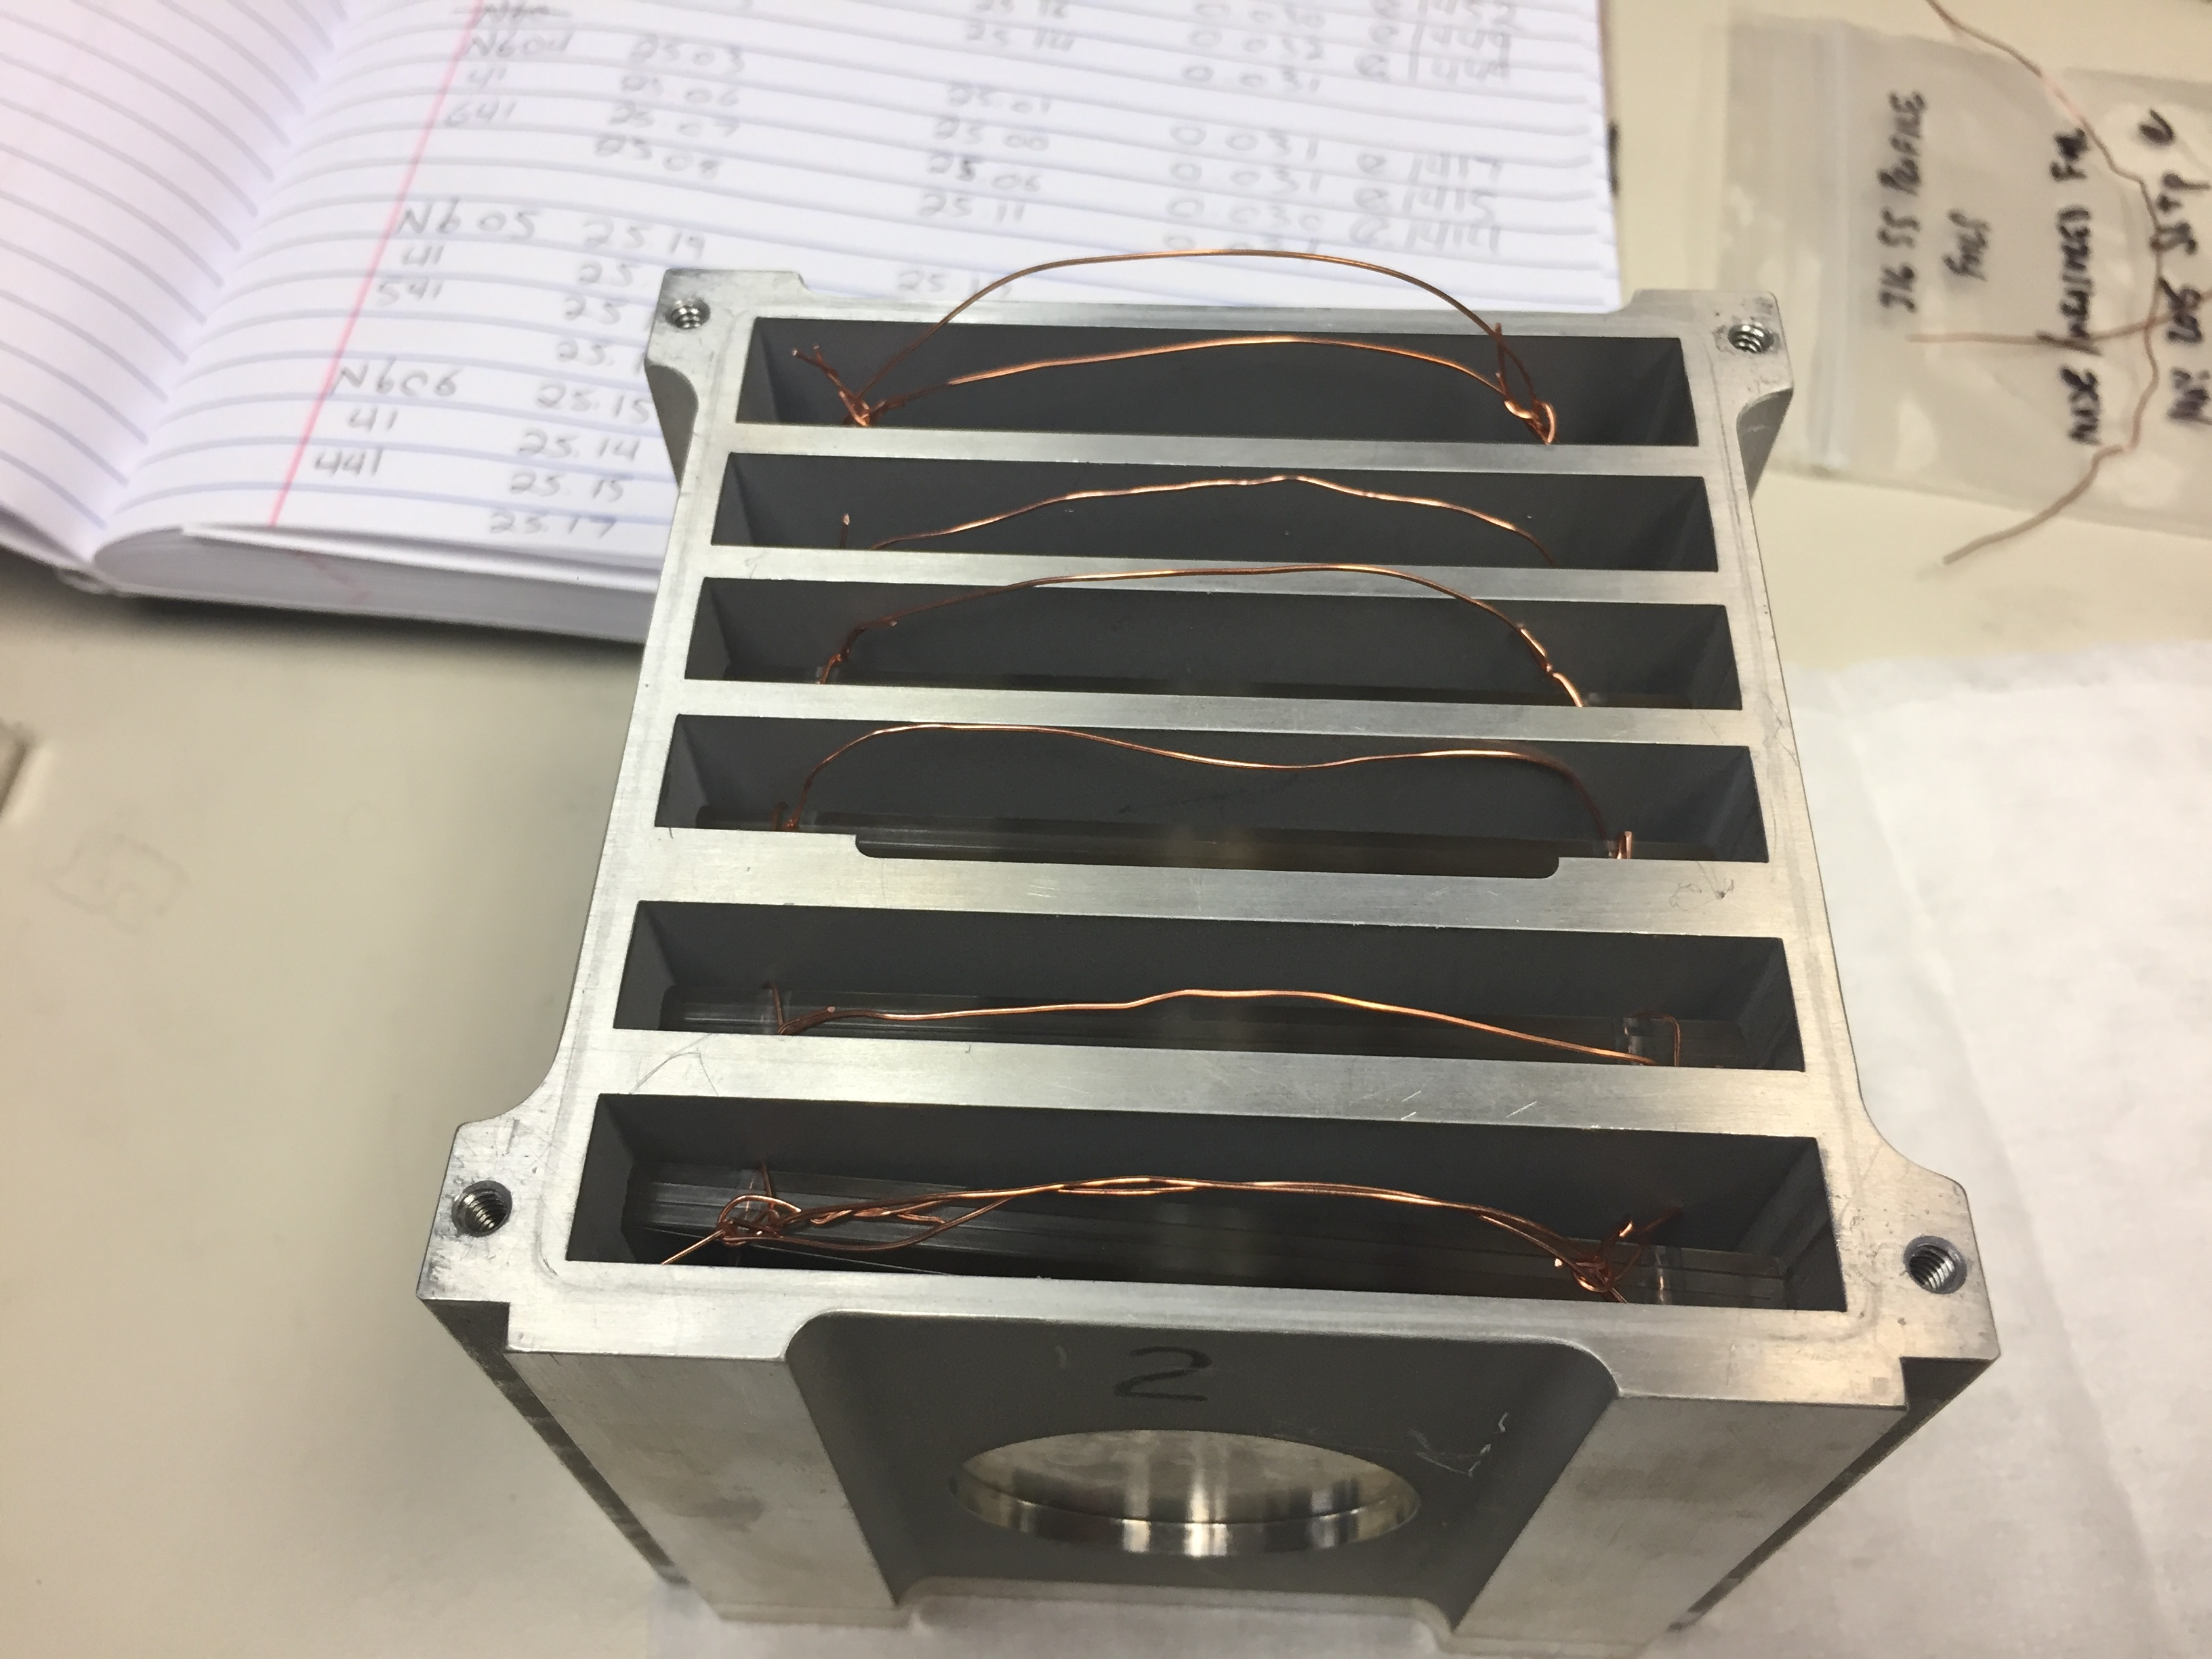
\includegraphics[scale=0.1,clip=true,trim=13cm 0cm 3cm 6cm]{./figures/IMG_1975.JPG}
 % IMG_1975.JPG: 3264x2448 pixel, 72dpi, 115.15x86.36 cm, bb=0 0 3264 2448
 \caption{Photograph of the assembled IPF target stack, before the stack's o-ring lid was sealed in place. The baling wire handles affixed to each bunch of Al+Cu+Nb foils are visible in each energy position, to facilitate removal of activated foils via robotic manipulators in the IPF hot cell. The circular Inconel beam entrance aperture is visible in the bottom center of the photograph.  }
 \label{fig:target_stack}
\end{figure}



% Please add the following required packages to your document preamble:
% \usepackage{booktabs}
\begin{table}[h]
\centering
\caption{Specifications of the  target stack design in the present work. The proton beam enters the stack upstream of the 249.8 \micro m SS profile monitor, and is transported through the stack in the order presented here. The 6061 aluminum degraders have a measured density of approximately 2.80 g/cm$^3$, but their areal densities are not listed here due to the variance minimization techniques described in this work.}
\label{tab:stack_table}
\begin{tabular}{@{}llll@{}}
\toprule
% Target Layer       & Nominal Thickness & Measured thickness (mg/cm\textasciicircum 2) & Thickness Uncertainty (\%) \\ \midrule
Target layer       & \begin{tabular}[c]{@{}l@{}}Measured \\ thickness\end{tabular} & \begin{tabular}[c]{@{}l@{}}Measured areal\\density (mg/cm$^2$)\end{tabular} & \begin{tabular}[c]{@{}l@{}}Areal density \\ uncertainty (\%)\end{tabular} \\ \midrule
SS profile monitor & 249.8 \micro m         & 194.555                                      & 0.290                      \\
Al-1               & 25.0 \micro m          & 6.519                                        & 0.724                      \\
Cu-1               & 61.3 \micro m          & 53.736                                       & 0.053                      \\
Nb-1               & 30.0 \micro m          & 23.205                                       & 0.073                      \\
Al Degrader 01     & 4.96 mm           & -                                            & -                          \\
Al-2               & 25.5 \micro m          & 6.484                                        & 0.364                      \\
Cu-2               & 61.8 \micro m          & 53.849                                       & 0.169                      \\
Nb-2               & 30.8 \micro m          & 22.905                                       & 0.166                      \\
Al Degrader 02     & 4.55 mm           & -                                            & -                          \\
Al-3               & 25.8 \micro m          & 6.472                                        & 0.314                      \\
Cu-3               & 61.5 \micro m          & 53.984                                       & 0.113                      \\
Nb-3               & 31.0 \micro m          & 22.906                                       & 0.235                      \\
Al Degrader 03     & 3.52 mm           & -                                            & -                          \\
Al-4               & 26.3 \micro m          & 6.505                                        & 0.407                      \\
Cu-4               & 61.3 \micro m          & 53.463                                       & 0.221                      \\
Nb-4               & 30.8 \micro m          & 22.550                                       & 0.245                      \\
Al Degrader 04     & 3.47 mm           & -                                            & -                          \\
Al-5               & 26.5 \micro m          & 6.479                                        & 0.296                      \\
Cu-5               & 61.5 \micro m          & 53.572                                       & 0.108                      \\
Nb-5               & 30.8 \micro m          & 22.110                                       & 0.248                      \\
Al Degrader 05     & 3.46 mm           & -                                            & -                          \\
Al-6               & 26.3 \micro m          & 6.475                                        & 0.624                      \\
Cu-6               & 62.0 \micro m          & 53.836                                       & 0.318                      \\
Nb-6               & 31.3 \micro m          & 22.120                                       & 0.130                      \\
SS profile monitor & 124.4 \micro m         & 101.336                                      & 0.226                      \\ \bottomrule
\end{tabular}
\end{table}





\subsection{Measurement of induced activities}\label{sec:spectroscopy}

XXXXXX



% \comment{Regex to replace table hard link with LaTeX cross-reference. - match w/ [T,t]able[^*}]   }


\subsection{Proton dosimetry}\label{sec:dosimetry}

% describe integral equation for converting activities to currents here

XXXXXX


\subsection{Proton transport calculations}\label{sec:proton_transport}

XXXXXX

% \begin{equation}
% R = N_T \int_0^{E_{max}} \sigma(E) \dfrac{d\phi}{dE} dE
% \end{equation}







\subsection{Calculation of measured cross sections}\label{sec:calcs_sec}

%  include 1st and 2nd order bateman stuff here

XXXXXX

 

% \begin{align}
% N_{\gamma} &= N_D \epsilon_\gamma I_\gamma \\
% &=  \epsilon_\gamma I_\gamma  \dfrac{N_T \sigma\pp{\bar{E}} \phi\pp{\bar{E}} }{\lambda}\pp{1 - e^{-\lambda t_i}}  e^{-\lambda t_d} \pp{1 - e^{-\lambda t_c}} \nonumber
% \end{align}



% \autoref{eqn:single_xs_eqn} can be used to determine the unknown (n,p) cross sections relative to the well-known \ce{^{115}In}(n,n')\ce{^{115m}In} and \ce{^{113}In}(n,n')\ce{^{113m}In} inelastic scattering cross sections since the Zn and Ti samples were co-irradiated with indium foils.
% This approach has a number of advantages since the result is independent of neutron flux and only depends on the relative detector efficiencies at each gamma-ray energy.
 

\subsection{Systematic uncertainties}

XXXXXX




\section{Results}


XXXXXX

          
% \section{Discussion}




% XXXXXX
 
 
 
 \section{Conclusions}

XXXXXX


 
 \section{Acknowledgements}
 
%  Stephen Graves - consulting for methodology, guidance.
 
 Michael Gallegos and Don Dry in the C-NR Countroom, David Reass and Mike Connors at IPF, and the LANSCE Accelerator Operations staff 
 
%  We would like to particularly point out the crucial role played by Cory Waltz in the design and commissioning of the HFNG.
%  We wish to thank Marc Garland and Saed Mirzadeh for discussions regarding the use of neutron generators for isotope production.
%  We acknowledge Glenn Jones of G\&J Jones Enterprises of Dublin, CA for the construction  of the High Flux Neutron Generator. 
%  Lastly, we would like to acknowledge the students in the Nuclear Reactions and Radiation (NE102) laboratory course at UC Berkeley who participated in these experiments, including Joe Corvino, Nizelle Fajardo, Scott Parker and Evan Still.  
%  
%  This work has been carried out at the University of California, Berkeley, and performed under the auspices of the U.S. Department of Energy by Lawrence Livermore National Laboratory under contract \# DE-AC52-07NA27344 and Lawrence Berkeley National Laboratory under contract \# DE-AC02-05CH11231.
% Funding has been provided from the US Nuclear Regulatory Commission, the US Nuclear Data Program, the Berkeley Geochronology Center, NSF ARRA Grant \# EAR-0960138, the University of California Laboratory Fees Research Grant \# 12-LR-238745, and  DFG Research Fellowship \# RU 2065/1-1.



% \pagebreak
% 
% \onecolumn
% 
\appendix


\section{Decay data} \label{data}
% 
% % \begin{longtable}{|c|c|c|c|c|} 
% % \caption{My caption}
% % \label{tab:dummy}
% % % \begin{tabular}{|c|c|c|c|c|}
% %    \hline
% %  
% % \end{longtable}
Table of decay data used for observed gamma rays. 
% 
% 
\section{Measured excitation functions} \label{fit_figures}

Plots of the cross sections measured in this work are presented here, in comparison with literature data and reaction modeling codes.
% 
% 
% % \begin{figure}[h]
% %  \centering
% %  \includegraphics[scale=0.7]{./hw04/fit110Ru240-cropped.pdf}
% %  % fit110Ru240.ps: 570x750 pixel, 72dpi, 20.11x26.46 cm, bb=0 0 570 750
% %  \caption{Fit to the \ce{^{110}Ru} 240.7 keV peak and its surroundings.}
% %  \label{fig:110Ru240}
% % \end{figure}
% % 

% \twocolumn

%% References with BibTeX database:

% \bibliographystyle{elsarticle-num}
% \bibliographystyle{elsarticle-harv}
% \bibliographystyle{elsarticle-num-names}
% \bibliography{<your-bib-database>}
% \addcontentsline{toc}{chapter}{Bibliography}
\bibliographystyle{elsarticle-num}
% \bibliographystyle{ieeetr}
\bibliography{../../library}
% \thispagestyle{fancyTOC}




%% Authors are advised to use a BibTeX database file for their reference list.
%% The provided style file elsarticle-num.bst formats references in the required Procedia style

%% For references without a BibTeX database:

% \begin{thebibliography}{00}

%% \bibitem must have the following form:
%%   \bibitem{key}...
%% 

% \bibitem{}

% \end{thebibliography}

\end{document}

%%
%% End of file `ecrc-template.tex'. 